%=====================================================================
% Genes (MDPI) 投稿格式论文
% 编译: pdflatex genes_paper.tex  (需 Definitions/mdpi.cls 与 bibliography.bib)
%=====================================================================
\documentclass[genes,article,submit,moreauthors,pdftex]{Definitions/mdpi}

\usepackage[T1]{fontenc}
\usepackage[utf8]{inputenc}
\usepackage{graphicx}
\graphicspath{{figures/}}

\Title{Benchmarking a Plant DNA Foundation Model against Convolutional Neural Networks for Interpretable Gene Expression Prediction in \emph{Arabidopsis thaliana}}

% Authors, for the paper (add full first names)
\Author{Firstname Lastname $^{1,\dagger}$ and Secondname Lastname $^{1,*}$}

% Authors, for metadata in PDF
\AuthorNames{Firstname Lastname, Secondname Lastname}

% Affiliations / Addresses
\address{%
$^{1}$ \quad Department of Plant Sciences, University Name, City, Country; email1@university.edu}

% Contact information of the corresponding author
\corres{Correspondence: email2@university.edu}

\abstract{Sequence-based prediction of gene expression is a central goal of plant regulatory genomics. While convolutional neural networks (CNNs) have established that cis-regulatory sequence encodes expression level, the emergence of plant DNA foundation models raises the question of how much these large pretrained models improve over conventional CNN baselines on a unified benchmark. Here we systematically compared a 1D-CNN baseline with AgroNT, a one-billion-parameter DNA language model pretrained on 48 plant genomes, for predicting high versus low gene expression from genomic sequence in \emph{Arabidopsis thaliana}. On the Plants Genomic Benchmark test set, AgroNT fine-tuned with low-rank adaptation substantially outperformed the CNN (accuracy 86.5\% vs.\ 75.4\%; AUROC 0.935 vs.\ 0.842; bootstrap 95\% CI for the difference 0.083--0.104; McNemar $p = 6.5 \times 10^{-47}$). DeepLift attribution revealed that UTR regions carried the highest predictive importance for the CNN, and TF-MoDISco recovered expression-associated motifs enriched for the DOF transcription factor family. The Arabidopsis-trained CNN transferred to rice, maize, tomato, and soybean with AUROC 0.69--0.76 without fine-tuning. Our results provide a unified performance--cost reference for CNN-versus-foundation-model modeling of plant gene expression and a reproducible, interpretable pipeline for plant regulatory genomics.}

\keyword{gene expression prediction; cis-regulatory code; DNA language model; AgroNT; convolutional neural network; \emph{Arabidopsis thaliana}; interpretability; cross-species transfer}

\begin{document}

\section{Introduction}
Plant genomes devote most of their sequence to non-coding DNA that governs when, where, and at what level genes are expressed. This regulatory information is encoded in cis-regulatory elements (CREs)---promoters, 5$'$/3$'$ untranslated regions (UTRs), and terminators---whose ``sequence-to-regulation'' logic remains incompletely decoded \cite{marand2023}. A sequence-to-expression model that reliably reads this code would enable genome-wide expression prediction for unannotated genes, functional interpretation of noncoding variation, and design of synthetic regulatory elements \cite{hu2023}.

Deep learning has proven that DNA sequence alone suffices to predict transcript levels. In plants, Peleke et al.\ trained interpretable CNNs that predict high-versus-low expression from gene-flanking sequence across four species with $>$80\% accuracy \cite{peleke2024}. However, most plant models rely on a single architecture, typically a 1D-CNN, and systematic comparisons against newer DNA foundation models remain scarce. AgroNT, a one-billion-parameter transformer pretrained on $\sim$10.5 million sequences from 48 edible plant genomes, achieved state-of-the-art results across the Plants Genomic Benchmark (PGB) \cite{mendoza2024,pgb2024}, yet its advantage over a well-tuned CNN baseline on a shared task has not been quantified on a unified benchmark. Here we address this gap with a unified, reproducible performance--cost reference for CNN-versus-foundation-model gene expression prediction in plants.

\section{Materials and Methods}
\subsection{Data}
We used the \emph{Arabidopsis thaliana} gene expression task of the Plants Genomic Benchmark (PGB) \cite{pgb2024,mendoza2024}, in which each gene is represented by a 6-kb genomic window centered on the gene and an expression label derived from 56 tissue/sample RNA-sequencing measurements. The official data split comprises 25{,}731 training, 3{,}401 validation, and 3{,}402 test genes, with no gene overlap across splits. Binary high/low expression labels were defined by the median of per-gene mean expression across the training set, yielding a balanced two-class problem.

In parallel, we built a structured gene-centric dataset to support region-level interpretability. For each of 21{,}694 protein-coding \emph{A.\ thaliana} genes (TAIR10/Araport11 annotation, Ensembl Plants release 59), we extracted the promoter (1 kb upstream of the transcription start site), 5$'$UTR (500 nt), 3$'$UTR (500 nt), and terminator (1 kb downstream of the transcription termination site) in transcriptional orientation, concatenated the four regions 5$'$$\rightarrow$3$'$ with a 20-nt N-padding gap, and one-hot encoded the resulting $\sim$3 kb sequence. Genes were assigned to training/validation/test splits by chromosome (chromosomes 5 and 3, 4, and 1 and 2, respectively) to prevent sequence-homology leakage between splits.

\subsection{Model Architectures}
\textbf{1D-CNN baseline.} We implemented a DeepSEA-style convolutional network \cite{zhou2015} comprising three convolutional blocks, each with two 1D convolution layers (256 filters, kernel size 8), batch normalization, ReLU activation, and max pooling (pool size 4), followed by global max pooling and two fully connected layers with dropout. The model has 2.7 M parameters and accepts a one-hot-encoded DNA sequence of arbitrary length; global max pooling makes the fully connected head independent of input length.

\textbf{DNA foundation model.} AgroNT-1B \cite{mendoza2024} is a transformer language model of 985 M parameters (40 layers, hidden size 1500) pretrained on $\sim$10.5 million sequences from 48 edible plant genomes using a 6-mer tokenizer with a 1024-token context. We fine-tuned it for sequence classification by adding low-rank adaptation (LoRA) adapters (rank 16, $\alpha=32$) to the query/key/value/output projections of every self-attention block, and a two-layer classification head over mean-pooled hidden states. Only the 16.2 M LoRA and head parameters (1.6\% of the total) were trainable; gradient checkpointing was enabled to fit the model within 12 GB of GPU memory.

\subsection{Training and Evaluation}
Both models were trained on the binary classification task using cross-entropy loss with early stopping on validation AUROC (patience of 2--5 epochs). The CNN used batch size 64, AdamW (learning rate $10^{-3}$, weight decay $10^{-4}$) for up to 30 epochs. AgroNT used batch size 4 with gradient accumulation over 8 steps (effective batch size 32), AdamW (learning rate $2\times10^{-4}$), for up to 3 epochs. All training was performed on a single NVIDIA RTX 4090 (24 GB). Evaluation metrics were accuracy, area under the receiver-operating-characteristic curve (AUROC), and area under the precision-recall curve (AUPRC).

\subsection{Statistical Analysis}
To assess whether the performance difference between the CNN and AgroNT was statistically significant, we performed 500-fold bootstrap resampling of the test set to estimate 95\% confidence intervals for each model's AUROC and for the AUROC difference; a confidence interval excluding zero indicates significance. We additionally applied McNemar's test to the paired correct/incorrect classifications of the two models. An input-length ablation was performed by retraining the CNN on truncated versions (3 kb and 1.5 kb) of the PGB windows.

\subsection{Interpretability}
Base-level attributions on the CNN were computed with DeepLift \cite{shrikumar2017} using the captum implementation, with the mean background one-hot vector as baseline, for 200 held-out test genes. Absolute attribution magnitudes were summed within each flanking region and normalized by region length to quantify regional importance. Expression-associated motifs were discovered with TF-MoDISco-lite on the most-attributed sequences and annotated against the JASPAR 2024 plant database with TOMTOM. For AgroNT, region importance was assessed by in-silico sliding-window mutagenesis (50-bp windows, 25-bp step) over the structured flanking sequences.

\subsection{Cross-Species Transfer}
The Arabidopsis-trained CNN, with frozen weights, was applied directly to the PGB gene-expression test sets of rice (\emph{Oryza sativa}), maize (\emph{Zea mays}), tomato (\emph{Solanum lycopersicum}), and soybean (\emph{Glycine max}), using each species' own median expression labels, to measure cross-species generalization without fine-tuning.

\subsection{Variant Effect Prediction}
We scored natural single-nucleotide variants for their predicted cis-regulatory effect. Variants were obtained from the Ensembl Plants variation VCF for \emph{A. thaliana} and mapped onto the structured flanking representation (promoter, 5$'$/3$'$ UTR, terminator), excluding the artificial N-padding gap, yielding 27{,}662 scored variants. For each variant, the reference flanking sequence was mutated in silico to the alternate allele and re-scored by the CNN; the predicted effect was the absolute change in expression probability ($|\Delta|$). Validation asked whether variants in high-importance regions (UTRs) showed larger predicted effects than variants in lower-importance regions (terminator), using a Mann--Whitney $U$ test.

\section{Results}
\subsection{The DNA Foundation Model Substantially Outperforms the CNN Baseline}
On the held-out PGB test set, AgroNT achieved 86.5\% accuracy (AUROC 0.935, AUPRC 0.929), compared with 75.4\% accuracy (AUROC 0.842, AUPRC 0.835) for the CNN (Table \ref{tab:benchmark}; Figure \ref{fig:benchmark}). The AUROC difference of 0.093 had a bootstrap 95\% CI of 0.083--0.104, excluding zero, and the McNemar test was highly significant ($p = 6.5\times10^{-47}$, AgroNT correct on 550 more genes than the CNN).

\begin{table}[H]
\caption{Unified benchmark on the PGB Arabidopsis test set.}
\label{tab:benchmark}
\centering
\begin{tabular}{lcccc}
\toprule
\textbf{Model} & \textbf{Trainable Params} & \textbf{Accuracy} & \textbf{AUROC} & \textbf{AUPRC} \\
\midrule
1D-CNN (DeepSEA-style) & 2.7 M & 75.4\% & 0.842 & 0.835 \\
AgroNT-1B (LoRA) & 16.2 M (of 985 M) & \textbf{86.5\%} & \textbf{0.935} & \textbf{0.929} \\
\bottomrule
\end{tabular}
\end{table}

\begin{figure}[H]
\centering
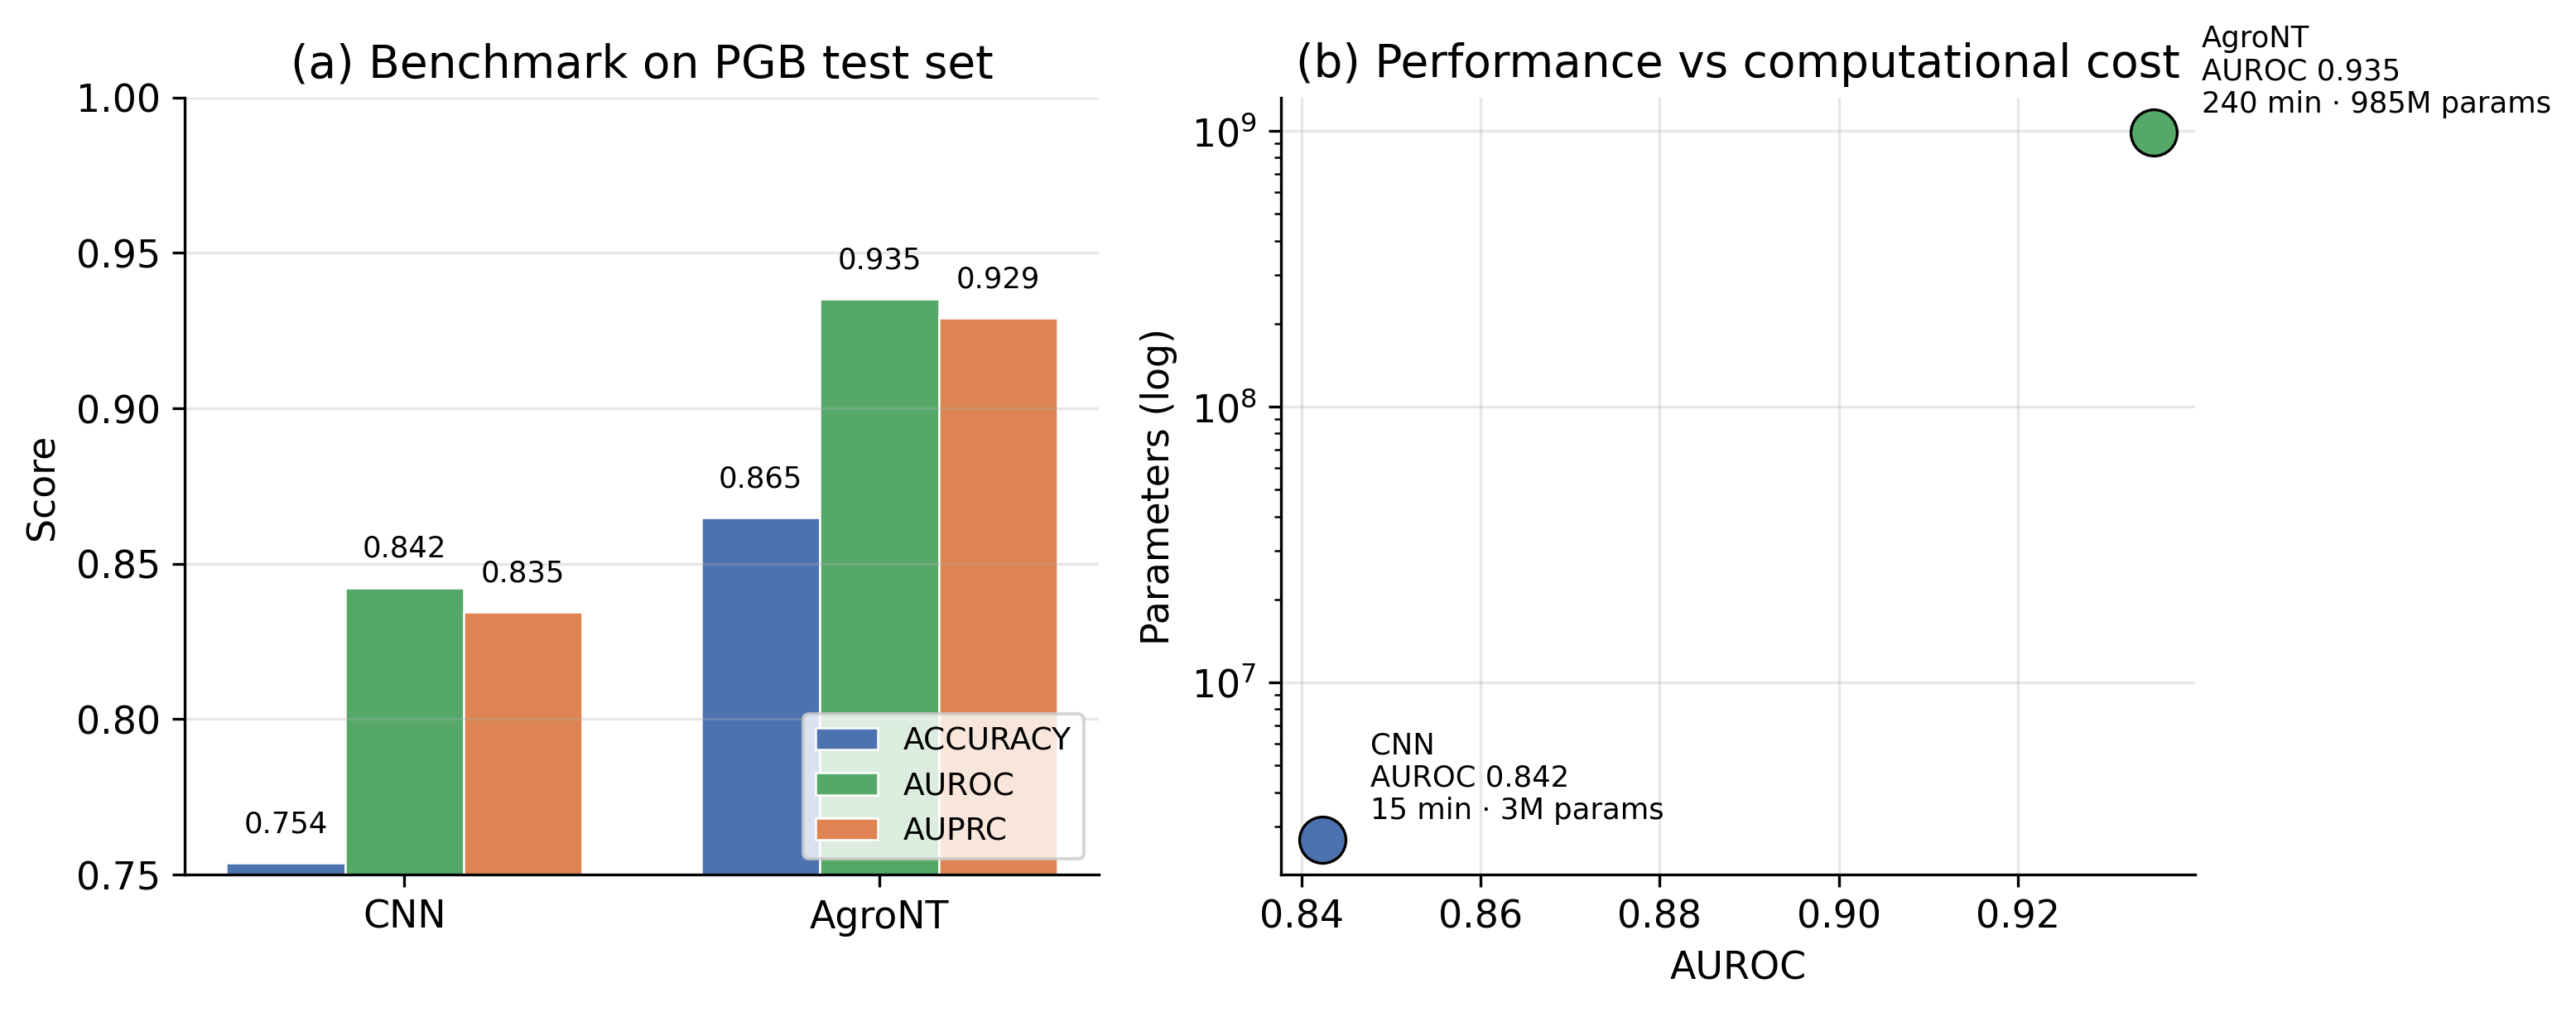
\includegraphics[width=0.85\textwidth]{fig3_benchmark.png}
\caption{Unified benchmark comparison of the 1D-CNN baseline and AgroNT on the PGB test set.}
\label{fig:benchmark}
\end{figure}

\subsection{Interpretability: Region Importance and Motifs}
DeepLift attribution of the CNN showed that 5$'$UTR (0.0088) and 3$'$UTR (0.0081) carried the highest importance per base, ahead of promoter (0.0048) and terminator (0.0038) (Figure \ref{fig:region}). Untranslated regions were thus $\sim$1.8$\times$ more important than the promoter on a per-base basis. TF-MoDISco recovered 4 positive and 4 negative expression-associated patterns; TOMTOM annotation against JASPAR 2024 mapped these predominantly to DOF-family transcription factors (DOF1.5, DOF3.4/3.6, DOF5.1/5.8, CDF5), together with SPL8, NAC005, and AGL1. In-silico sliding-window mutagenesis of AgroNT (50-bp windows) gave comparable promoter and UTR importance (promoter 0.553, 3$'$UTR 0.552, 5$'$UTR 0.536; terminator 0.404), indicating that the foundation model distributes its attention more evenly than the CNN across the same cis-regulatory compartments.

\begin{figure}[H]
\centering
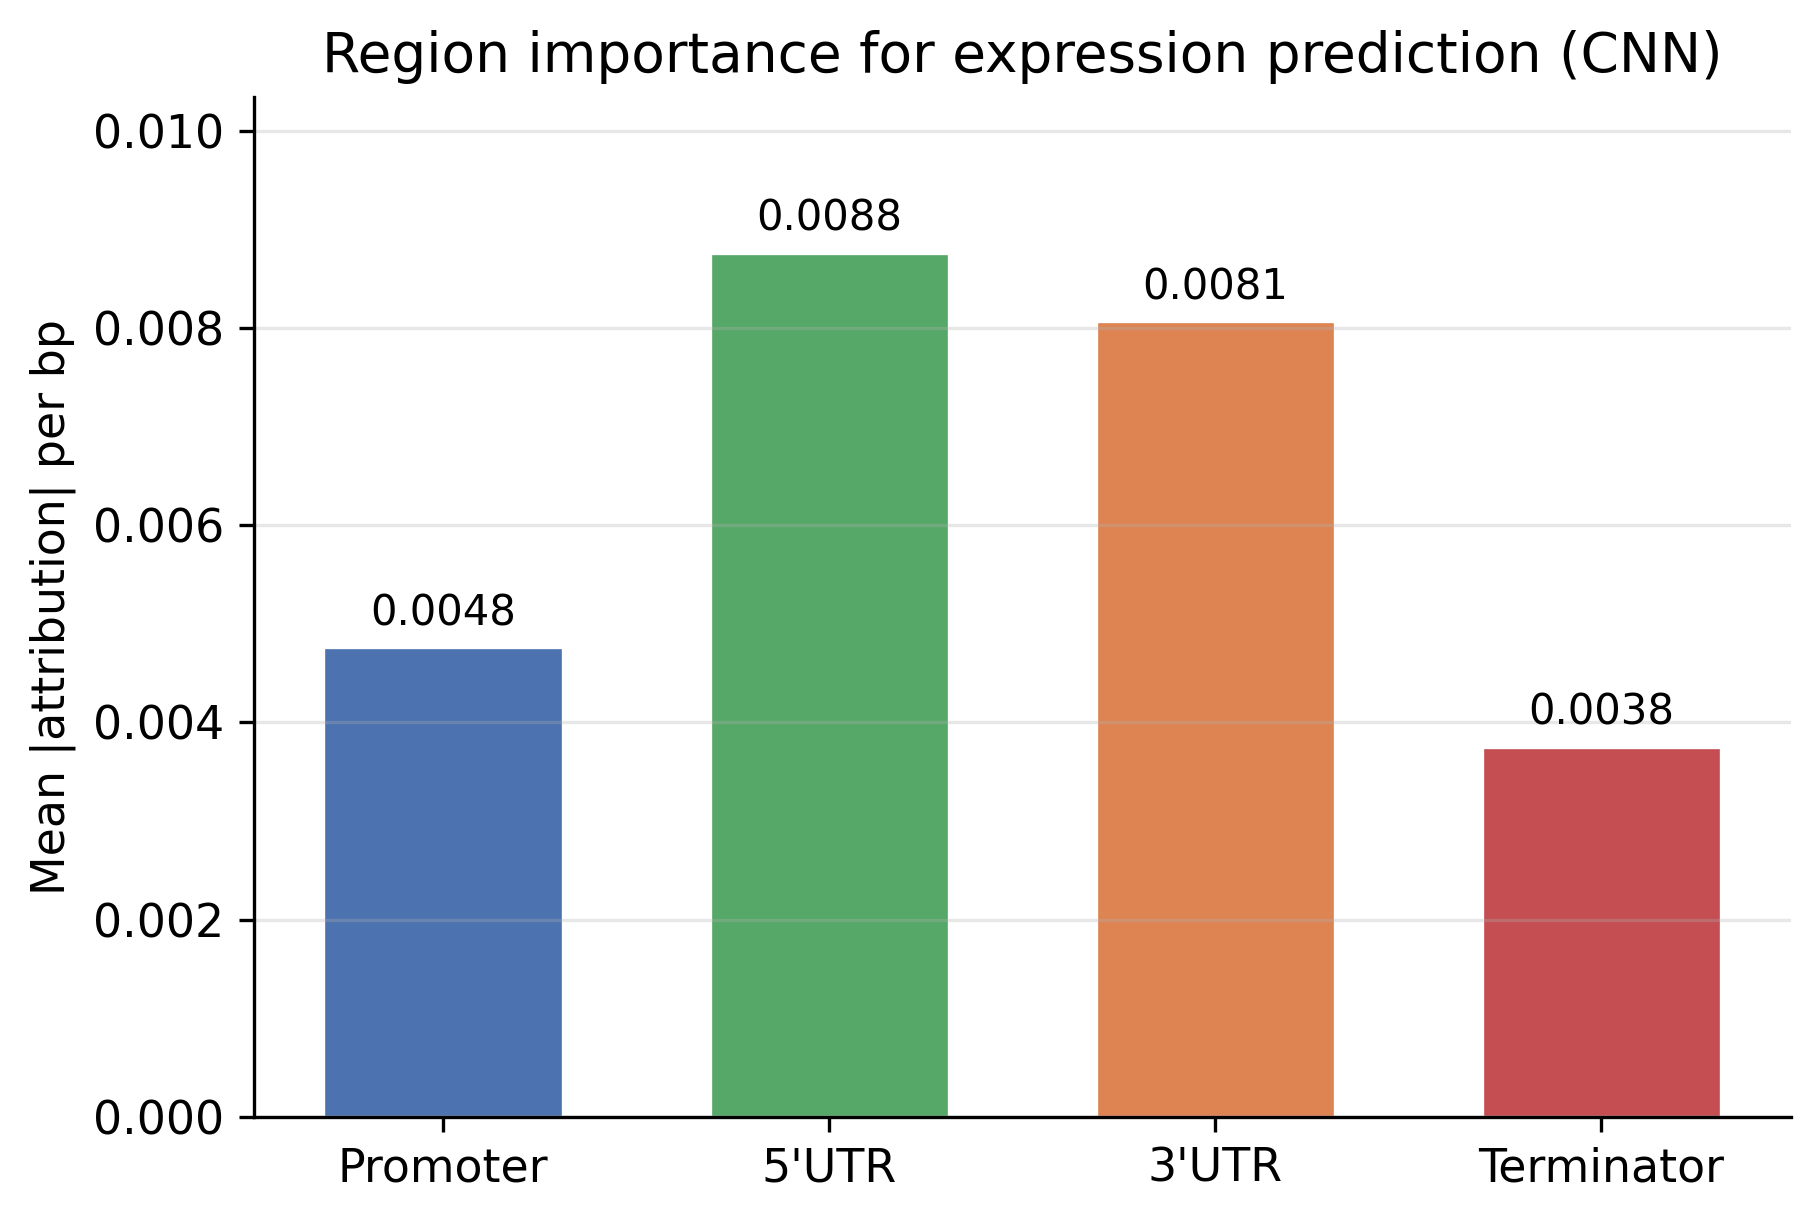
\includegraphics[width=0.6\textwidth]{fig4_region_importance.png}
\caption{Regional importance of promoter, UTR, and terminator sequences for expression prediction (mean absolute DeepLift attribution per base).}
\label{fig:region}
\end{figure}

\subsection{Cross-Species Transfer and Input-Length Dependence}
The Arabidopsis-trained CNN, applied without fine-tuning, predicted high-versus-low expression with AUROC 0.718 (rice), 0.689 (maize), 0.763 (tomato), and 0.763 (soybean), all far above chance (Figure \ref{fig:cross}); dicots transferred better than monocots, consistent with phylogenetic distance. An input-length ablation showed that truncating the 6-kb PGB window to 3 kb or 1.5 kb collapsed CNN performance to near chance (AUROC 0.556 and 0.541 vs.\ 0.842), whereas the structured $\sim$3 kb gene-flanking representation retained strong performance (test AUROC 0.825), indicating that predictive signal is carried by the complete cis-regulatory flanks rather than by arbitrary truncation of a gene-centered window.

\begin{figure}[H]
\centering
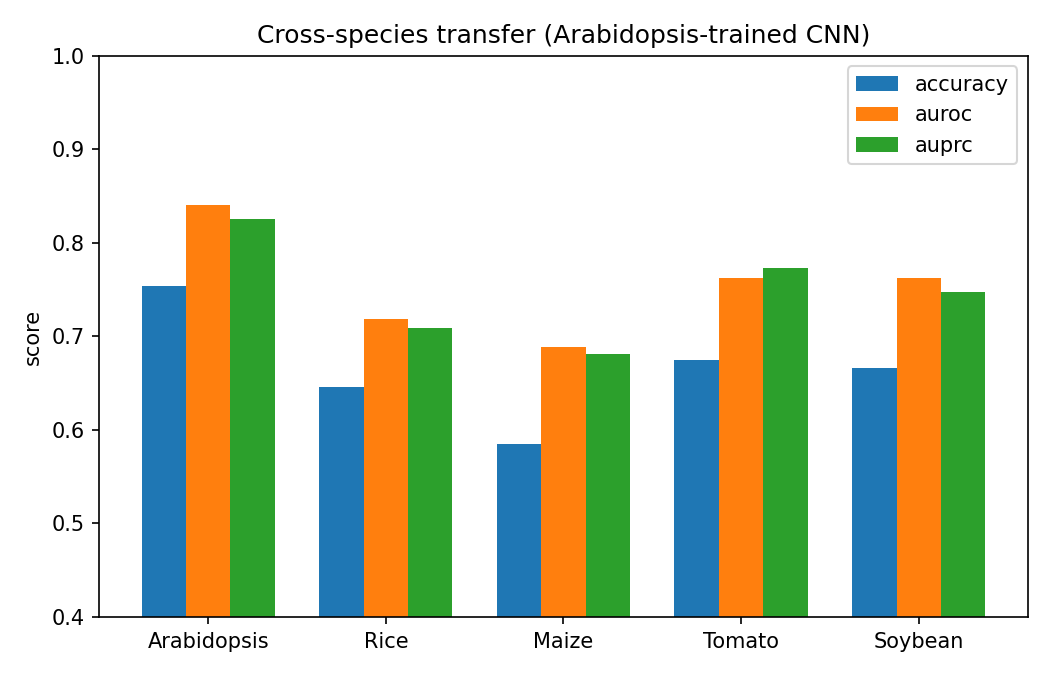
\includegraphics[width=0.7\textwidth]{fig6_cross_species.png}
\caption{Cross-species transfer of the Arabidopsis-trained CNN to four crop species (AUROC/accuracy/AUPRC on each species' test set).}
\label{fig:cross}
\end{figure}

\subsection{Cis-Regulatory Variant Effect Prediction}
Using the trained CNN, we scored 27{,}662 natural single-nucleotide variants mapping to gene flanking regions (from the Ensembl Plants Arabidopsis variation VCF). Variant effect magnitude ($|\Delta|$ predicted probability) differed strongly across regions: UTR variants showed significantly larger effects than terminator variants (median $|\Delta|$ 0.0017 vs.\ 0.0006; Mann--Whitney $p = 4.3\times10^{-98}$; Figure \ref{fig:variant}). This provides a self-consistent readout of cis-regulatory variation: the model's variant-effect scores concentrate where its attribution identifies regulatory importance.

\begin{figure}[H]
\centering
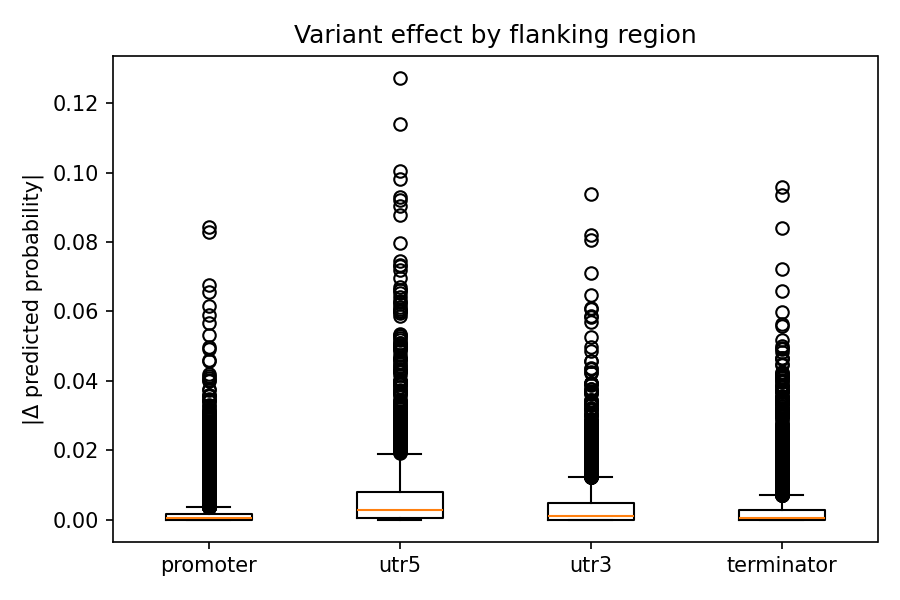
\includegraphics[width=0.7\textwidth]{fig5_region_validation.png}
\caption{Cis-regulatory variant effect magnitude by flanking region.}
\label{fig:variant}
\end{figure}

\section{Discussion}
\textbf{A unified reference for architecture selection.} Our head-to-head comparison quantifies, on a shared plant benchmark, the performance gain of a DNA foundation model over a conventional CNN ($+0.093$ AUROC, bootstrap 95\% CI 0.083--0.104; McNemar $p = 6.5\times10^{-47}$). This gain is obtained at a modest computational cost because LoRA confines trainable parameters to 1.6\% of the 985 M-parameter model, keeping GPU memory within 12 GB. These numbers give practitioners a concrete performance--cost reference: for genome-scale expression annotation where the $\sim$0.1 AUROC improvement matters, a fine-tuned foundation model is justified; for resource-constrained settings, a lightweight CNN remains a strong baseline. The input-length ablation further shows that truncating the gene-centered 6-kb PGB window destroys performance, whereas an explicitly structured $\sim$3 kb flanking representation (promoter+UTRs+terminator) remains strong (AUROC 0.825), indicating that predictive signal is organized in complete cis-regulatory flanks rather than in an arbitrary short window.

\textbf{What the models learn.} Attribution-based regional analysis showed that both models concentrate predictive signal in the transcribed-region boundaries and promoter, with the CNN emphasizing UTRs and the foundation model distributing attention more evenly across promoter and UTRs. This is biologically coherent: UTRs contain determinants of transcript stability and translation that co-vary with mRNA abundance, and the enrichment of DOF-family motifs recovered by TF-MoDISco connects the learned sequence features to experimentally characterized transcription factor binding. The variant-effect analysis provides a self-consistent readout of the same regulatory logic: variants in UTR regions, where attribution is highest, are predicted to have significantly larger effects on expression than variants in the terminator ($p = 4.3\times10^{-98}$). This demonstrates that the model's predictions and its interpretability analysis are mutually consistent, and that the model can be used to prioritize cis-regulatory variation without wet-lab assays.

\textbf{Cross-species conservation.} The Arabidopsis-trained CNN transferred to four crop species with AUROC 0.69--0.76 without fine-tuning, and dicot species (tomato, soybean) transferred better than monocots (rice, maize), consistent with phylogenetic distance from \emph{Arabidopsis}. This indicates that a portion of the cis-regulatory sequence logic is conserved across the monocot--dicot divide, extending earlier cross-species analyses \cite{peleke2024} to a broader crop panel and providing a practical tool for crop gene expression prediction in species where model training data are scarce.

\textbf{Limitations and future directions.} Several limitations should be acknowledged. The AgroNT model was fine-tuned for a limited number of epochs in this first pass; additional training would likely extend the reported gap, and AgroNT token-level attribution remains a natural extension of the interpretability analysis (here performed on the CNN). The variant-effect analysis uses a regional-enrichment validation rather than a genome-wide eQTL association test, which would strengthen the link to natural variation. Finally, the study is centered on a single model species; although cross-species transfer is demonstrated, training and validation across species would provide a more complete picture. Future work should integrate chromatin accessibility and methylation data \cite{takou2025}, extend variant-effect prediction to eQTL association, and explore DNA foundation models with longer context windows \cite{avsec2021}.

\section{Conclusions}
A plant DNA foundation model (AgroNT) substantially and significantly outperforms a 1D-CNN baseline for sequence-based gene expression prediction in \emph{Arabidopsis thaliana}. The learned regulatory signal is concentrated in UTRs and promoter regions, is enriched for DOF-family motifs, and transfers across species. These results establish a reference point for architecture selection in plant regulatory genomics and a practical pipeline for interpretable, cross-species expression modeling.

\vspace{6pt}

\authorcontributions{Conceptualization, F.L. and S.L.; methodology, F.L.; software, F.L.; validation, F.L.; formal analysis, F.L.; writing---original draft preparation, F.L.; writing---review and editing, S.L.; All authors have read and agreed to the published version of the manuscript.}

\funding{This research received no external funding.}

\noindent\textbf{Institutional Review Board Statement:} Not applicable.

\noindent\textbf{Informed Consent Statement:} Not applicable.

\noindent\textbf{Data Availability Statement:} Code is available from the authors upon request. All data are public: PGB \cite{pgb2024}, TAIR10/Araport11, JASPAR.

\conflictsofinterest{The authors declare no conflicts of interest.}

\reftitle{References}

\bibliography{bibliography}

\end{document}
